\documentclass[11pt]{article}
\usepackage{ctex}
\usepackage[english]{babel}
\usepackage{blindtext}
\usepackage{nameref}
\usepackage{fancyhdr}
\usepackage{amsmath,amssymb,amsthm}
\usepackage{graphicx,float}
\usepackage{physics}
\usepackage{pgfplots}
\usepackage[a4paper, total={6in, 9in}]{geometry}

\graphicspath{{../images/}}

\pagestyle{fancy}
\fancyhf{}
\fancyhf[HL]{F4 期末練習試題}
\fancyhf[CF]{\thepage}

\newcommand{\innerprod}[2]{\langle{#1},{#2}\rangle}
\newcommand{\id}{\mathtt{id}}

\newtheorem*{definition}{Definition}
\newtheorem*{theorem}{Theorem}
\newtheorem*{corollary}{Corollary}
\newtheorem*{lemma}{Lemma}
\newtheorem*{proposition}{Proposition}
\newtheorem*{remark}{Remark}
\newtheorem*{claim}{Claim}
\newtheorem*{example}{Example}
\newtheorem*{axiom}{Axiom}

\begin{document}
    \thispagestyle{plain}

    \centering 

    \section*{練習試卷\\數學必修部分\\試題-答題簿}

    \raggedright

    \subsection*{規則}

    \begin{enumerate}
        \item 此試卷必須使用中文回答。
        \item 除特別指明外,需詳細列出所有算式。
        \item 除特別指明外,數值答案必須用真確值表示。
        \item 本試卷只作\textbf{内部使用}。
        \item 所有試題取自AL/CE/DSE歷届試題,來源: https://www.dse.life/ppindex/m2/
    \end{enumerate}
    \newpage

    \begin{enumerate}
        \item 設$f(x)=\dfrac{1}{2}x-\dfrac{1}{144}x^2-6$。運用配方法,求$y=f(x)$的圖像的頂點坐標。
        
            \hrulefill
                
            \hrulefill
            
            \hrulefill
        
            \hrulefill
            
            \hrulefill
                
            \hrulefill
            
            \hrulefill
                
            \hrulefill
            
            \hrulefill
            
            \hrulefill
            
            \hrulefill
            
            \hrulefill
            
            \hrulefill
            
            \hrulefill
            
            \hrulefill
            
            \hrulefill
            
            \hrulefill
            
            \hrulefill
            
            \hrulefill
            
            \hrulefill
            
            \hrulefill
            
            \hrulefill
            
            \hrulefill
            
            \hrulefill
            
            \hrulefill
            
            \hrulefill
            
            \hrulefill
            
            \hrulefill
            
            \hrulefill

        \pagebreak
        \item 設$C(k)$ 為 $y=\dfrac{1}{k+1}[2x^2+(k+7)x+4]$的圖像,其中 $k\neq -1$.\begin{enumerate}
            \item 若 $C(k)$ 的兩個x軸截距為 $P$ 和 $Q$,同時 $PQ=1$,求$k$的值。
            \item 求 $k$ 的值的範圍使得 $C(k)$ 沒有x軸截距。
            \item \begin{enumerate}
                \item 求 $C(1)$ 和 $C(2)$的交點。
                \item 證明對於任意$k$, $C(k)$ 都穿過 (c)(i) 的兩個交點。 
            \end{enumerate} 
        \end{enumerate}
        
            \hrulefill
                
            \hrulefill
            
            \hrulefill
            
            \hrulefill
            
            \hrulefill
            
            \hrulefill
            
            \hrulefill
            
            \hrulefill
            
            \hrulefill
            
            \hrulefill
            
            \hrulefill
            
            \hrulefill
            
            \hrulefill
            
            \hrulefill
            
            \hrulefill
            
            \hrulefill
            
            \hrulefill
            
            \hrulefill
            
            \hrulefill
            
            \hrulefill
            
            \hrulefill
            
            \hrulefill
            
            \hrulefill

        \pagebreak
        \item \begin{enumerate}
            \item 設 $f(x)=36x-x^2$。運用配方法,求 $y=f(x)$的圖像的頂點。
            \item 繩子的長度為 108m。某保安將之分成兩段。其中一段圍繞成一個面積爲 $A$ m$^2$的長方形。另一段則劃分長方形為兩個區域,如圖所示。\begin{figure}[H]
                \centering
                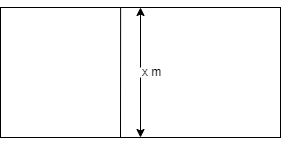
\includegraphics[scale=0.4]{f4finalq3.png}
            \end{figure}\begin{enumerate}
                \item 試以$x$表述 $A$。
                \item 該保安認爲長方形的面積可超過 500 m$^{2}$。你同意嗎?試加以解釋。
            \end{enumerate}
        \end{enumerate}
        
            \hrulefill
                
            \hrulefill

            \hrulefill
            
            \hrulefill
        
            \hrulefill
            
            \hrulefill
                
            \hrulefill
            
            \hrulefill
                
            \hrulefill
            
            \hrulefill
            
            \hrulefill
            
            \hrulefill
            
            \hrulefill

            \hrulefill
            
            \hrulefill
        
            \hrulefill
            
            \hrulefill
                
            \hrulefill
            
            \hrulefill
            
            \hrulefill
            
            \hrulefill
            
            \hrulefill
        
            \hrulefill
            
            \hrulefill
                
            \hrulefill
            
            \hrulefill
                
            \hrulefill
            
            \hrulefill
            
            \hrulefill
            
            \hrulefill
            
            \hrulefill
            
            \hrulefill
            
            \hrulefill
            
            \hrulefill
            
            \hrulefill
            
            \hrulefill
            
            \hrulefill
            
            \hrulefill
            
            \hrulefill
            
            \hrulefill
            
            \hrulefill
            
            \hrulefill
            
            \hrulefill
            
            \hrulefill
            
            \hrulefill
            
            \hrulefill
            
            \hrulefill
            
            \hrulefill

        \pagebreak
        \item 如圖所示,$ABCD$爲一個棱形。其對角綫$AC$與$BD$相交於$E$。\begin{figure}[H]
            \centering
            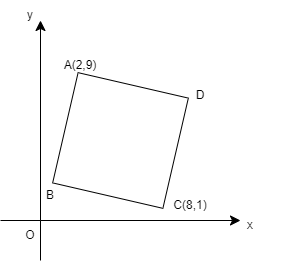
\includegraphics[scale=0.6]{f4finalq4.png}
        \end{figure}\begin{enumerate}
            \item 求\begin{enumerate}
                \item $E$的坐標;
                \item $BD$的直綫方程。
            \end{enumerate}
            \item 已知$AD$的直綫方程為$x+7y-65=0$。求\begin{enumerate}
                \item $BC$的直綫方程;
                \item $AB$的長度。
            \end{enumerate}
        \end{enumerate}

            \hrulefill
                    
            \hrulefill

            \hrulefill
            
            \hrulefill
        
            \hrulefill
            
            \hrulefill
                
            \hrulefill
            
            \hrulefill
                
            \hrulefill
            
            \hrulefill
            
            \hrulefill
            
            \hrulefill
            
            \hrulefill

            \hrulefill
            
            \hrulefill
        
            \hrulefill
            
            \hrulefill
                
            \hrulefill
            
            \hrulefill
            
            \hrulefill
            
            \hrulefill
            
            \hrulefill
        
            \hrulefill
            
            \hrulefill
                
            \hrulefill
            
            \hrulefill
                
            \hrulefill
            
            \hrulefill
            
            \hrulefill
            
            \hrulefill
            
            \hrulefill
            
            \hrulefill
            
            \hrulefill
            
            \hrulefill
            
            \hrulefill
            
            \hrulefill
            
            \hrulefill
            
            \hrulefill
            
            \hrulefill
            
            \hrulefill
            
            \hrulefill
            
            \hrulefill
            
            \hrulefill
            
            \hrulefill
            
            \hrulefill

        \pagebreak
        \item 如圖所示,穿過 $A$ 與 $B$的直綫垂直於穿過$A$ 和 $C$的直綫,其中 $C$ 為x軸上的一點。\begin{figure}[H]
            \centering
            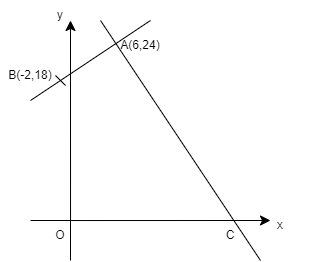
\includegraphics[scale=0.6]{f4finalq5.png}
        \end{figure}\begin{enumerate}
            \item 求穿過 $A$ 和 $B$的直綫方程。
            \item 求 $C$的坐標。
            \item 求$\triangle ABC$的面積。
            \item 現有直綫穿過 $A$ 與$D$,$D$為 $BC$上的一點, 使得$\triangle ABD$的面積為 90 平方單位。 設 $BD:DC=r:1$。求 $r$的值。
        \end{enumerate}
        \hrulefill
                    
            \hrulefill

            \hrulefill
            
            \hrulefill
        
            \hrulefill
            
            \hrulefill
                
            \hrulefill
            
            \hrulefill
                
            \hrulefill
            
            \hrulefill
            
            \hrulefill
            
            \hrulefill
            
            \hrulefill

            \hrulefill
            
            \hrulefill
        
            \hrulefill
            
            \hrulefill
                
            \hrulefill
            
            \hrulefill
            
            \hrulefill
            
            \hrulefill
            
            \hrulefill
        
            \hrulefill
            
            \hrulefill
                
            \hrulefill
            
            \hrulefill
                
            \hrulefill
            
            \hrulefill
            
            \hrulefill
            
            \hrulefill
            
            \hrulefill
            
            \hrulefill
            
            \hrulefill
            
            \hrulefill
            
            \hrulefill
            
            \hrulefill
            
            \hrulefill
            
            \hrulefill
            
            \hrulefill
            
            \hrulefill
            
            \hrulefill
            
            \hrulefill
            
            \hrulefill
            
            \hrulefill
            
            \hrulefill

        \pagebreak
        \item \begin{enumerate}
            \item 因式分解 $a^4-16$ 和 $a^3-8$.
            \item 求 $a^4-16$ 和 $a^3-8$的L.C.M.
        \end{enumerate}
        \hrulefill
            
            \hrulefill
            
            \hrulefill
            
            \hrulefill
            
            \hrulefill
            
            \hrulefill
            
            \hrulefill
            
            \hrulefill
            
            \hrulefill
            
            \hrulefill
            
            \hrulefill
            
            \hrulefill
            
            \hrulefill
            
            \hrulefill
            
        \item 因式分解\begin{enumerate}
            \item $m^2+12mn+36n^2$.
            \item $m^2+12mn+36n^2-s^2$.
        \end{enumerate}
        \hrulefill
            
            \hrulefill
            
            \hrulefill
            
            \hrulefill
            
            \hrulefill
            
            \hrulefill
            
            \hrulefill
            
            \hrulefill
            
            \hrulefill
            
            \hrulefill
            
            \hrulefill

        \pagebreak
        \item 因式分解\begin{enumerate}
            \item $x^3+x^2y-7x^2$.
            \item $x^3+x^2y-7x^2-x-y+7$.
        \end{enumerate}
        \hrulefill
            
            \hrulefill
            
            \hrulefill
            
            \hrulefill
            
            \hrulefill
            
            \hrulefill
            
            \hrulefill
            
            \hrulefill
            
            \hrulefill
            
            \hrulefill
            
            \hrulefill

        \item 因式分解\begin{enumerate}
            \item $4m^2-9$.
            \item $2m^2n+7mn-15n$.
            \item $4m^2-9-2m^2n-7mn+15n$
        \end{enumerate}
        \hrulefill
            
            \hrulefill
            
            \hrulefill
            
            \hrulefill
            
            \hrulefill
            
            \hrulefill
            
            \hrulefill
            
            \hrulefill
            
            \hrulefill
            
            \hrulefill
            
            \hrulefill

        \pagebreak
        \item 已知 $f(x)=2x^2+ax+b$。\begin{enumerate}
            \item 若 $f(x)$ 被 $(x-1)$所除,所得餘數為 $-5$。若 $f(x)$ 被 $(x+2)$所除,所得餘數為 4。 求 $a$ 和 $b$的值。
            \item 若$f(x)=0$,求$x$的值。
        \end{enumerate}
        \hrulefill
            
            \hrulefill
            
            \hrulefill
            
            \hrulefill
            
            \hrulefill
            
            \hrulefill
            
            \hrulefill
            
            \hrulefill
            
            \hrulefill
            
            \hrulefill
            
            \hrulefill

            \hrulefill
            
            \hrulefill
            
            \hrulefill
            
            \hrulefill

            \hrulefill
            
            \hrulefill
            
            \hrulefill
            
            \hrulefill
            
            \hrulefill
            
            \hrulefill
            
            \hrulefill
            
            \hrulefill
            
            \hrulefill
            
            \hrulefill

        \pagebreak
        \item 若 $3x^2-kx-2$ 可被 $x-k$整除,求 $k$的兩個可能值。
            
            \hrulefill
                
            \hrulefill
            
            \hrulefill
            
            \hrulefill
            
            \hrulefill
            
            \hrulefill
            
            \hrulefill
            
            \hrulefill
            
            \hrulefill
            
            \hrulefill
            
            \hrulefill
            
            \hrulefill
            
            \hrulefill
            
            \hrulefill
            
            \hrulefill
            
            \hrulefill

            \hrulefill
            
            \hrulefill
            
            \hrulefill
            
            \hrulefill

            \hrulefill
            
            \hrulefill
            
            \hrulefill
            
            \hrulefill
            
            \hrulefill
            
            \hrulefill
            
            \hrulefill
            
            \hrulefill
            
            \hrulefill
            
            \hrulefill

        \pagebreak
        \item \begin{enumerate}
            \item 求 $5x^3+12x^2-9x-7$ 被 $x^2+2x-3$所除時的餘數。
            \item 設 $g(x)=(5x^3+12x^2-9x-7)-(ax+b)$,其中 $a$ 和 $b$ 為常數。 已知 $g(x)$ 可被 $x^2+2x-3$整除。\begin{enumerate}
                \item 寫出 $a$ 和 $b$的值。
                \item 解方程 $g(x)=0$。
            \end{enumerate}
        \end{enumerate}

        \hrulefill
                
            \hrulefill
            
            \hrulefill
            
            \hrulefill
            
            \hrulefill
            
            \hrulefill
            
            \hrulefill
            
            \hrulefill
            
            \hrulefill
            
            \hrulefill
            
            \hrulefill
            
            \hrulefill
            
            \hrulefill
            
            \hrulefill
            
            \hrulefill
            
            \hrulefill

            \hrulefill
            
            \hrulefill
            
            \hrulefill
            
            \hrulefill

            \hrulefill
            
            \hrulefill
            
            \hrulefill
            
            \hrulefill
            
            \hrulefill
            
            \hrulefill
            
            \hrulefill
            
            \hrulefill
            
            \hrulefill
            
            \hrulefill

            \hrulefill
                
            \hrulefill
            
            \hrulefill
            
            \hrulefill
            
            \hrulefill
            
            \hrulefill
            
            \hrulefill
            
            \hrulefill
            
            \hrulefill
            
            \hrulefill
            
            \hrulefill
            
            \hrulefill
            
            \hrulefill
            
            \hrulefill
            
            \hrulefill
            
            \hrulefill

            \hrulefill
            
            \hrulefill
            
            \hrulefill
            
            \hrulefill

            \hrulefill
            
            \hrulefill
            
            \hrulefill
            
            \hrulefill
            
            \hrulefill

        \pagebreak
        \item 簡化以下算式,并以正指數表示。\begin{enumerate}
            \item $\dfrac{x^3y^2}{x^{-3}y}$.
            \item $x(\dfrac{x^{-1}}{y^2})^{-3}$.
            \item $\dfrac{(m^5n^{-2})^6}{m^4n^{-3}}$.
        \end{enumerate}

        \hrulefill
            
            \hrulefill
            
            \hrulefill
            
            \hrulefill
            
            \hrulefill
            
            \hrulefill
            
            \hrulefill
            
            \hrulefill
            
            \hrulefill
            
            \hrulefill

            \hrulefill
                
            \hrulefill
            
            \hrulefill
            
            \hrulefill
            
            \hrulefill
            
            \hrulefill
            
            \hrulefill
            
            \hrulefill
            
            \hrulefill
            
            \hrulefill
            
            \hrulefill
            
            \hrulefill
            
            \hrulefill
            
            \hrulefill

        \pagebreak
        \item 簡化 $\sqrt{\dfrac{3^{5k+2}}{27^k}}$.
        
        \hrulefill
            
            \hrulefill
            
            \hrulefill
            
            \hrulefill
            
            \hrulefill
            
            \hrulefill
            
            \hrulefill
            
            \hrulefill
            
            \hrulefill
            
            \hrulefill
            
            \hrulefill
            
            \hrulefill
            
            \hrulefill

        \item 簡化 $\dfrac{\log(a^2)+\log(b^4)}{\log(ab^2)}$,其中 $a,b>0$。
        
        \hrulefill
            
            \hrulefill
            
            \hrulefill
            
            \hrulefill
            
            \hrulefill
            
            \hrulefill
            
            \hrulefill
            
            \hrulefill
            
            \hrulefill
            
            \hrulefill
            
            \hrulefill
            
            \hrulefill
            
            \hrulefill

        \pagebreak
        \item 設 $\log{2}=x, \log{3}=y$。試以$x$和$y$表述以下數值。\begin{enumerate}
            \item $\log{18}$.
            \item $\log{15}$.
            \item $\log{\sqrt{12}}$.
        \end{enumerate}

        \hrulefill
            
            \hrulefill
            
            \hrulefill
            
            \hrulefill
            
            \hrulefill
            
            \hrulefill
            
            \hrulefill
            
            \hrulefill
            
            \hrulefill
            
            \hrulefill
            
            \hrulefill
            
            \hrulefill
            
            \hrulefill

        \item 不使用計算機,計算以下數值:\begin{enumerate}
            \item $3^x=\dfrac{1}{\sqrt{27}}$;
            \item $\log{x}+2\log{4}=\log{48}$.
        \end{enumerate}

        \hrulefill
            
            \hrulefill
            
            \hrulefill
            
            \hrulefill
            
            \hrulefill
            
            \hrulefill
            
            \hrulefill
            
            \hrulefill
            
            \hrulefill
            
            \hrulefill

        \pagebreak
        \item 某研究員運用度量 $A$ 和度量 $B$ 去描述爆炸强度,如下表:
        \begin{center}
            \begin{tabular}{ |c|c| }
                \hline
                度量&公式\\
                \hline
                $A$&$M=\log_4{E}$\\
                \hline
                $b$&$M=\log_8{E}$\\
                \hline
            \end{tabular}
        \end{center}
        已知 $M$ 和 $N$ 分別爲度量 $A$ 和度量 $B$ 所計算的爆炸强度,而$E$ 是爆炸所釋放的能量。 若以度量 $B$計算的爆炸强度為6.4,求度量$A$所計算的爆炸强度。

        \hrulefill
            
            \hrulefill
            
            \hrulefill
            
            \hrulefill
            
            \hrulefill
            
            \hrulefill
            
            \hrulefill
            
            \hrulefill
            
            \hrulefill
            
            \hrulefill

            \hrulefill
            
            \hrulefill
            
            \hrulefill
            
            \hrulefill
            
            \hrulefill
            
            \hrulefill
            
            \hrulefill
            
            \hrulefill
            
            \hrulefill
            
            \hrulefill

        \pagebreak
        \item 設 $a$ 和$b$ 為常數。記 $y=a+\log_b{x}$ 的圖像為 $G$。若$G$的x軸截距為 9 而且 $G$ 通過 $(243,3)$。試以$y$表述 $x$。
        
        \hrulefill
            
            \hrulefill
            
            \hrulefill
            
            \hrulefill
            
            \hrulefill
            
            \hrulefill
            
            \hrulefill
            
            \hrulefill
            
            \hrulefill
            
            \hrulefill

            \hrulefill
            
            \hrulefill
            
            \hrulefill
            
            \hrulefill
            
            \hrulefill
            
            \hrulefill
            
            \hrulefill
            
            \hrulefill
            
            \hrulefill
            
            \hrulefill
            
            \hrulefill
            
            \hrulefill
            
            \hrulefill
            
            \hrulefill
            
            \hrulefill
            
            \hrulefill
            
            \hrulefill
            
            \hrulefill

        \pagebreak
        \item 解:\begin{enumerate}
            \item $\displaystyle\begin{cases}
                4^{x-y}=4\\
                4^{x+y}=16
            \end{cases}$,求 $x$ 和 $y$的值。
            \item $3^{2x}+3^x-2=0$,求 $x$的值。
            \item $\log_3(x-3)+\log_3(x+3)=3$,求 $x$的值。
        \end{enumerate}

        \hrulefill
            
            \hrulefill
            
            \hrulefill
            
            \hrulefill
            
            \hrulefill

            \hrulefill
            
            \hrulefill
            
            \hrulefill
            
            \hrulefill
            
            \hrulefill
            
            \hrulefill
            
            \hrulefill

        \item 若 $2\log_{10}{x}-\log_{10}{y}=0$。證明 $y=x^2$。
            
            \hrulefill
            
            \hrulefill
            
            \hrulefill
            
            \hrulefill
            
            \hrulefill
            
            \hrulefill
            
            \hrulefill
            
            \hrulefill
            
            \hrulefill
            
            \hrulefill
            
            \hrulefill

        \pagebreak
        \item 解以下方程:\begin{enumerate}
            \item $1-2x=\sqrt{2-x}$.
            \item $x-\sqrt{x+1}=5$.
            \item $x-5\sqrt{x}-6=0$.
        \end{enumerate}

        \hrulefill
            
            \hrulefill
            
            \hrulefill
            
            \hrulefill
            
            \hrulefill
            
            \hrulefill
            
            \hrulefill
            
            \hrulefill
            
            \hrulefill
            
            \hrulefill
            
            \hrulefill

            \hrulefill
            
            \hrulefill
            
            \hrulefill
            
            \hrulefill
            
            \hrulefill
            
            \hrulefill
            
            \hrulefill
            
            \hrulefill
            
            \hrulefill
            
            \hrulefill
            
            \hrulefill

        \pagebreak
        \item 求 $k$的值的範圍使得 $2x^2+x+5=k(x+1)^2$ 沒有實數解。
        
        \hrulefill
            
            \hrulefill
            
            \hrulefill
            
            \hrulefill
            
            \hrulefill
            
            \hrulefill
            
            \hrulefill
            
            \hrulefill
            
            \hrulefill
            
            \hrulefill
            
            \hrulefill

        \item 若二次方程 $x^2-6x+2k=0$ 及 $x^2-5x+k$ 有共同根 $\alpha$。 (即 $\alpha$ 同時為兩方程的解) 證明 $\alpha=k$ 並求出$k$的值。
        
        \hrulefill

            \hrulefill
            
            \hrulefill
            
            \hrulefill
            
            \hrulefill
            
            \hrulefill
            
            \hrulefill
            
            \hrulefill
            
            \hrulefill
            
            \hrulefill
            
            \hrulefill
            
            \hrulefill

        \pagebreak
        \item 設 $\alpha$和 $\beta$ 為 $x^2+kx+1=0$ 的根,其中 $k$ 為常數。\begin{enumerate}
            \item 求以下數值,並以$k$表述答案:\begin{enumerate}
                \item $(\alpha+2)+(\beta+2)$,
                \item $(\alpha+2)(\beta+2)$.
            \end{enumerate}
            \item 設 $\alpha+2$ 和 $\beta+2$ 為$x^2+px+q=0$的解其中 $p$ 和 $q$ 為常數。 求 $p$ 和 $q$的值,並以$k$表述答案。
        \end{enumerate}

        \hrulefill

            \hrulefill
            
            \hrulefill
            
            \hrulefill
            
            \hrulefill
            
            \hrulefill
            
            \hrulefill
            
            \hrulefill
            
            \hrulefill
            
            \hrulefill
            
            \hrulefill
            
            \hrulefill

            \hrulefill

            \hrulefill
            
            \hrulefill
            
            \hrulefill
            
            \hrulefill
            
            \hrulefill
            
            \hrulefill
            
            \hrulefill
            
            \hrulefill
            
            \hrulefill
            
            \hrulefill
            
            \hrulefill

        \pagebreak
        \item 若$\displaystyle \frac{1}{m}+\frac{1}{n}=\frac{1}{a}$ 及 $m+n=b$,試以$a$ 和 $b$表述下列表達式:\begin{enumerate}
            \item $mn$,
            \item $m^2+n^2$.
        \end{enumerate}

        \hrulefill

            \hrulefill
            
            \hrulefill
            
            \hrulefill
            
            \hrulefill
            
            \hrulefill
            
            \hrulefill
            
            \hrulefill
            
            \hrulefill
            
            \hrulefill

        \item 設 $\alpha$ 和 $\beta$ 為 $kx^2-4x+2k=0$的根,其中 $k$ ($k\neq 0$) 為常數。 試以 $k$表述下列表達式:\begin{enumerate}
            \item $\alpha^2+\beta^2$,
            \item $\dfrac{\alpha}{\beta}+\dfrac{\beta}{\alpha}$.
        \end{enumerate}

        \hrulefill

            \hrulefill
            
            \hrulefill
            
            \hrulefill
            
            \hrulefill
            
            \hrulefill
            
            \hrulefill
            
            \hrulefill
            
            \hrulefill
            
            \hrulefill
            
            \hrulefill
            
            \hrulefill

        \pagebreak
        \item 以$a+bi$的形式表達 $\dfrac{1}{1+2i}$,其中$a$ 和 $b$ 為實數。
        
        \hrulefill

            \hrulefill
            
            \hrulefill
            
            \hrulefill
            
            \hrulefill
            
            \hrulefill
            
            \hrulefill
            
            \hrulefill
            
            \hrulefill
            
            \hrulefill
            
            \hrulefill
            
            \hrulefill

        \item 若 $a:b=3:4$ 和 $a:c=2:5$,求\begin{enumerate}
            \item $a:b:c$,
            \item $\dfrac{ac}{a^2+b^2}$的值。
        \end{enumerate}

        \hrulefill

            \hrulefill
            
            \hrulefill
            
            \hrulefill
            
            \hrulefill
            
            \hrulefill
            
            \hrulefill
            
            \hrulefill
            
            \hrulefill
            
            \hrulefill
            
            \hrulefill
            
            \hrulefill

        \pagebreak
        \item 某游樂場中,成人比兒童的人數為$13:6$。若9名成人及24名兒童進入游樂場,則新的成人比兒童的人數為$8:7$。求原本成人的數量。
        
        \hrulefill

            \hrulefill
            
            \hrulefill
            
            \hrulefill
            
            \hrulefill
            
            \hrulefill
            
            \hrulefill
            
            \hrulefill
            
            \hrulefill
            
            \hrulefill
            
            \hrulefill
            
            \hrulefill

        \item 已知 $z$ 正變於 $x^2$ 並反變於 $y$。當$x=1$ 及 $y=2$時,則$z=3$。求當$x=2$ 及 $y=3$時,$z$的值。
        
        \hrulefill

            \hrulefill
            
            \hrulefill
            
            \hrulefill
            
            \hrulefill
            
            \hrulefill
            
            \hrulefill
            
            \hrulefill
            
            \hrulefill
            
            \hrulefill
            
            \hrulefill
            
            \hrulefill

        \pagebreak
        \item 某變量 $y$ 可拆分爲兩部分。首部分正變於 $x$而另一部分正變於$x^2$。 當$x=1$時 , $y=-5$; 當 $x=2$時, $y=-8$。\begin{enumerate}
            \item 試以$x$表述$y$。
            \item 由此,當$x=6$時,求 $y$的值 。
        \end{enumerate}

        \hrulefill

            \hrulefill
            
            \hrulefill
            
            \hrulefill
            
            \hrulefill
            
            \hrulefill
            
            \hrulefill
            
            \hrulefill
            
            \hrulefill
            
            \hrulefill
            
            \hrulefill
            
            \hrulefill

            \hrulefill

            \hrulefill
            
            \hrulefill
            
            \hrulefill
            
            \hrulefill
            
            \hrulefill
            
            \hrulefill
            
            \hrulefill
            
            \hrulefill
            
            \hrulefill
            
            \hrulefill
            
            \hrulefill

        \pagebreak
        \item 某工廠中,一張周界為 $s$ 米的地毯的成本為 $\$C$。已知$C$為兩部分的和,一部分正變於 $s$ 同時另一部分正變於 $s$的平方。當 $s=2$時, $C=356$; 當$s=5$時, $C=1250$。\begin{enumerate}
            \item 求一張周界為6米的地毯的成本。
            \item 若地毯的成本為 $\$539$,求地毯的周界。
        \end{enumerate}

        \hrulefill

            \hrulefill
            
            \hrulefill
            
            \hrulefill
            
            \hrulefill
            
            \hrulefill
            
            \hrulefill
            
            \hrulefill
            
            \hrulefill
            
            \hrulefill
            
            \hrulefill
            
            \hrulefill

            \hrulefill

            \hrulefill
            
            \hrulefill
            
            \hrulefill
            
            \hrulefill
            
            \hrulefill
            
            \hrulefill
            
            \hrulefill
            
            \hrulefill
            
            \hrulefill
            
            \hrulefill
            
            \hrulefill

        \pagebreak
        \item 已知 $h(x)$ 部分為常數同時部分正變於 $x$。設 $h(-2)=-96$及$h(5)=72$。\begin{enumerate}
            \item 求 $h(x)$。
            \item 解方程 $h(x)=3x^2$。
        \end{enumerate}

        \hrulefill
            
            \hrulefill
            
            \hrulefill
            
            \hrulefill
            
            \hrulefill
            
            \hrulefill
            
            \hrulefill
            
            \hrulefill
            
            \hrulefill
            
            \hrulefill
            
            \hrulefill

            \hrulefill

            \hrulefill
            
            \hrulefill
            
            \hrulefill
            
            \hrulefill
            
            \hrulefill
            
            \hrulefill
            
            \hrulefill
            
            \hrulefill
            
            \hrulefill
            
            \hrulefill
            
            \hrulefill

        \pagebreak
        \item 簡化下列表達式:\begin{enumerate}
            \item $\dfrac{1-\cos^2{x}}{\sin{x}}$.
            \item $\dfrac{\sin(180^\circ-\theta)}{\sin(90^\circ+\theta)}$.
            \item $\sin^2(180^\circ-\phi)+\sin^2(270^\circ+\phi)$.
        \end{enumerate}

        \hrulefill

            \hrulefill

            \hrulefill
            
            \hrulefill
            
            \hrulefill
            
            \hrulefill
            
            \hrulefill
            
            \hrulefill
            
            \hrulefill
            
            \hrulefill

        \item 解下列方程,其中 $0^\circ\leq \theta< 360^\circ$。答案取值三位有效數字。\begin{enumerate}
            \item $\sin^2{\theta}+7\sin^2{\theta}=5\cos^2{\theta}$.
            \item $\sin^2{\theta}-3\cos{\theta}-1=0$.
        \end{enumerate}

        \hrulefill

        \hrulefill
            
        \hrulefill
        
        \hrulefill
        
        \hrulefill
        
        \hrulefill
        
        \hrulefill
        
        \hrulefill
        
        \hrulefill
        
        \hrulefill
        
        \hrulefill
        
        \hrulefill

    \pagebreak
    \item 圖中,船 $A$ 和船 $B$ 從燈塔 $L$觀察到的方位角分別為 $020^\circ$及 $110^\circ$。$B$在 $A$的$140^\circ$ 20 公里處。\begin{figure}[H]
        \centering
        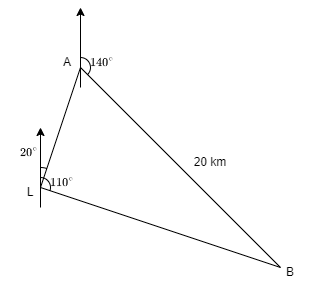
\includegraphics[scale=0.6]{f4finalq37.png}
    \end{figure}求 \begin{enumerate}
        \item $B$與 $L$的距離;
        \item $L$ 對 $B$的方位角。
    \end{enumerate}

    \hrulefill

        \hrulefill
            
        \hrulefill
        
        \hrulefill
        
        \hrulefill
        
        \hrulefill
        
        \hrulefill
        
        \hrulefill
        
        \hrulefill
        
        \hrulefill
        
        \hrulefill
        
        \hrulefill

        \hrulefill

        \hrulefill
            
        \hrulefill
        
        \hrulefill
        
        \hrulefill
        
        \hrulefill
        
        \hrulefill
        
        \hrulefill
        
        \hrulefill
        
        \hrulefill
        
        \hrulefill
        
        \hrulefill

        \hrulefill

        \hrulefill
            
        \hrulefill
        
        \hrulefill
        
        \hrulefill
        
        \hrulefill
        
        \hrulefill
        
        \hrulefill
        
        \hrulefill
        
        \hrulefill
        
        \hrulefill
        
        \hrulefill
            
        \hrulefill
        
        \hrulefill
        
        \hrulefill
        
        \hrulefill
        
        \hrulefill
        
        \hrulefill
        
        \hrulefill
        
        \hrulefill
        
        \hrulefill
        
        \hrulefill

    \pagebreak
    \item 圖中 $AB=4$, $AC=5$ and $BC=7$。求 $\angle A$ 至最接近的度。\begin{figure}[H]
        \centering
        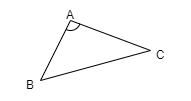
\includegraphics[scale=0.8]{f4finalq38.png}
    \end{figure}

    \hrulefill
        
        \hrulefill
            
        \hrulefill
        
        \hrulefill
        
        \hrulefill
            
        \hrulefill
        
        \hrulefill

    \item 如圖所示,求 $AB$ 及 $\triangle ABC$的面積。\begin{figure}[H]
        \centering
        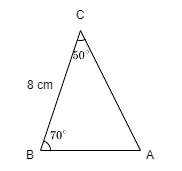
\includegraphics[scale=0.8]{f4finalq39.png}
    \end{figure}

    
        
        \hrulefill
            
        \hrulefill
        
        \hrulefill
        
        \hrulefill
        
        \hrulefill
        
        \hrulefill
        
        \hrulefill
        
        \hrulefill

    \pagebreak
    \item 如圖所示, $ABC$ 為等邊三角形。 $AB=2$。 $D,E,F$ 分別爲 $AB,BC,CA$ 上的點,使得 $AD=BE=CF=x$。\begin{figure}[H]
        \centering
        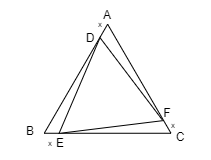
\includegraphics[scale=0.8]{f4finalq40.png}
    \end{figure}\begin{enumerate}
        \item 運用餘弦定理或其他方法,以$x$表述 $DE^2$ 。
        \item 證明 $\triangle DEF$的面積爲$\dfrac{\sqrt{3}}{4}(3x^2-6x+4)$。
    \end{enumerate}
    \hrulefill
            
        \hrulefill
        
        \hrulefill
        
        \hrulefill
        
        \hrulefill
        
        \hrulefill
        
        \hrulefill
        
        \hrulefill
        
        \hrulefill
        
        \hrulefill
        
        \hrulefill
            
        \hrulefill
        
        \hrulefill
        
        \hrulefill
        
        \hrulefill
        
        \hrulefill
        
        \hrulefill
        
        \hrulefill
        
        \hrulefill
        
        \hrulefill
        
        \hrulefill

        \hrulefill
        
        \hrulefill
        
        \hrulefill
        
        \hrulefill
        
        \hrulefill
        
        \hrulefill
        
        \hrulefill
        
        \hrulefill
        
        \hrulefill
        
        \hrulefill
            
        \hrulefill
        
        \hrulefill
        
        \hrulefill
        
        \hrulefill
        
        \hrulefill
        
        \hrulefill
        
        \hrulefill
        
        \hrulefill
        
        \hrulefill
        
        \hrulefill
        
        \hrulefill
        
        \hrulefill
        
        \hrulefill
        
        \hrulefill
            
        \hrulefill
        
        \hrulefill
        
        \hrulefill
        
        \hrulefill

    \pagebreak
    \end{enumerate}
\end{document}